\begin{activity}{5}
The image below illustrates how the linear transformation
$T : \IR^2 \rightarrow \IR^2$ given by the
standard matrix $A = \begin{bmatrix} 2 & 0 \\ 0 & 3 \end{bmatrix}$
transforms the unit square.

\begin{center}
\begin{tikzpicture}[scale=0.5]
\fill[red!50!white] (0,0) rectangle (1,1);`
\draw[thin,gray,<->] (-4,0)-- (4,0);
\draw[thin,gray,<->] (0,-4)-- (0,4);
\draw[thick,blue,->] (0,0) -- node[below] {$A \vec{e}_1= \begin{bmatrix}2 \\ 0 \end{bmatrix}$}++ (2,0);
\draw[thick,blue,->] (0,0) -- node[left] {$A \vec{e}_2 = \begin{bmatrix} 0 \\ 3 \end{bmatrix}$}++(0,3);
\draw[thick,red,->] (0,0) -- ++(1,0);
\draw[thick,red,->] (0,0) -- ++(0,1);
\draw[blue,dashed] (2,0) -- (2,3) -- (0,3);
\draw[red,dashed] (1,0) -- (1,1) -- (0,1);
\end{tikzpicture}
\end{center}

\begin{enumerate}[(a)]
\item What are the lengths of \(A\vec e_1\) and \(A\vec e_2\)?
\item What is the area of the transformed unit square?
\end{enumerate}

\end{activity}


\begin{activity}{5}
The image below illustrates how the linear transformation
$S : \IR^2 \rightarrow \IR^2$ given by the
standard matrix $B = \begin{bmatrix} 2 & 3 \\ 0 & 4 \end{bmatrix}$.
transforms the unit square.

\begin{center}
\begin{tikzpicture}[scale=0.5]
\fill[red!50!white] (0,0) rectangle (1,1);
\draw[thin,gray,<->] (-4,0)-- (4,0);
\draw[thin,gray,<->] (0,-4)-- (0,4);
\draw[thick,blue,->] (0,0) -- node[below] {$B \vec{e}_1= \begin{bmatrix}2 \\ 0 \end{bmatrix}$}++ (2,0);
\draw[thick,blue,->] (0,0) -- ++(3,4) node[above] {$B \vec{e}_2 = \begin{bmatrix} 3 \\ 4 \end{bmatrix}$};
\draw[thick,red,->] (0,0) -- ++(1,0);
\draw[thick,red,->] (0,0) -- ++(0,1);
\draw[blue,dashed] (2,0) -- (5,4) -- (3,4);
\draw[red,dashed] (1,0) -- (1,1) -- (0,1);
\end{tikzpicture}
\end{center}

\begin{enumerate}[(a)]
\item What are the lengths of \(B\vec e_1\) and \(B\vec e_2\)?
\item What is the area of the transformed unit square?
\end{enumerate}
\end{activity}

\begin{observation}
  It is possible to find two nonparallel vectors that are scaled but not rotated by
  the linear map given by \(B\).

\begin{multicols}{2}
  \[B\vec e_1=\begin{bmatrix} 2 & 3 \\ 0 & 4 \end{bmatrix}\begin{bmatrix}1\\0\end{bmatrix}
  =\begin{bmatrix}2\\0\end{bmatrix}=2\vec e_1\]

  \[
    B\begin{bmatrix}\frac{3}{4}\\\frac{1}{2}\end{bmatrix}
      =
    \begin{bmatrix} 2 & 3 \\ 0 & 4 \end{bmatrix}\begin{bmatrix}\frac{3}{4}\\\frac{1}{2}\end{bmatrix}
      =
    \begin{bmatrix}3\\2\end{bmatrix}
      =
    4\begin{bmatrix}\frac{3}{4}\\\frac{1}{2}\end{bmatrix}
  \]

\columnbreak

  \begin{center}
  \begin{tikzpicture}[scale=0.5]
  \fill[red!50!white] (0,0) -- (1,0) -- (1.75,0.5) -- (0.75,0.5) -- (0,0);
  \draw[thin,gray,<->] (-4,0)-- (4,0);
  \draw[thin,gray,<->] (0,-4)-- (0,4);
  \draw[thick,blue,->] (0,0) -- node[below] {$B\begin{bmatrix}1\\0\end{bmatrix}=2\begin{bmatrix}1\\0\end{bmatrix}$}++ (2,0);
  \draw[thick,blue,->] (0,0) -- ++(3,2) node[above] {$B\begin{bmatrix}\frac{3}{4}\\\frac{1}{2}\end{bmatrix}=4\begin{bmatrix}\frac{3}{4}\\\frac{1}{2}\end{bmatrix}$};
  \draw[thick,red,->] (0,0) -- (1,0);
  \draw[thick,red,->] (0,0) -- (0.75,0.5);
  \draw[red,dashed] (1,0) -- (1.75,0.5) -- (0.75,0.5);
  \draw[blue,dashed] (2,0) -- (5,2) -- (3,2);
  \end{tikzpicture}
  \end{center}
\end{multicols}

  The process for finding such vectors will be covered later in this module.
\end{observation}


\begin{observation}
  Notice that while a linear map can transform vectors in various ways,
  linear maps always transform parallelograms into parallelograms,
  and these areas are always transformed by the same factor: in the case of
  \(B=\begin{bmatrix} 2 & 3 \\ 0 & 4 \end{bmatrix}\),
  this factor is \(8\).
\begin{center}
\begin{tikzpicture}[scale=0.5]
\fill[red!50!white] (0,0) rectangle (1,1);
\draw[thin,gray,<->] (-4,0)-- (4,0);
\draw[thin,gray,<->] (0,-4)-- (0,4);
\draw[thick,blue,->] (0,0) -- node[below] {$B \vec{e}_1= \begin{bmatrix}2 \\ 0 \end{bmatrix}$}++ (2,0);
\draw[thick,blue,->] (0,0) -- ++(3,4) node[above] {$B \vec{e}_2 = \begin{bmatrix} 3 \\ 4 \end{bmatrix}$};
\draw[thick,red,->] (0,0) -- ++(1,0);
\draw[thick,red,->] (0,0) -- ++(0,1);
\draw[blue,dashed] (2,0) -- (5,4) -- (3,4);
\draw[red,dashed] (1,0) -- (1,1) -- (0,1);
\end{tikzpicture}
  \begin{tikzpicture}[scale=0.5]
  \fill[red!50!white] (0,0) -- (1,0) -- (1.75,0.5) -- (0.75,0.5) -- (0,0);
  \draw[thin,gray,<->] (-4,0)-- (4,0);
  \draw[thin,gray,<->] (0,-4)-- (0,4);
  \draw[thick,blue,->] (0,0) -- node[below] {$B\begin{bmatrix}1\\0\end{bmatrix}=2\begin{bmatrix}1\\0\end{bmatrix}$}++ (2,0);
  \draw[thick,blue,->] (0,0) -- ++(3,2) node[above] {$B\begin{bmatrix}\frac{3}{4}\\\frac{1}{2}\end{bmatrix}=4\begin{bmatrix}\frac{3}{4}\\\frac{1}{2}\end{bmatrix}$};
  \draw[thick,red,->] (0,0) -- (1,0);
  \draw[thick,red,->] (0,0) -- (0.75,0.5);
  \draw[red,dashed] (1,0) -- (1.75,0.5) -- (0.75,0.5);
  \draw[blue,dashed] (2,0) -- (5,2) -- (3,2);
  \end{tikzpicture}
\end{center}
Since this change in area is always the same for a given linear map,
it will be equal to the value of the transformed unit square (which
begins with area \(1\)).
\end{observation}

\begin{remark}
We will define the \term{determinant} of a square matrix \(A\),
or \(\det(A)\) for short, to be the factor by which \(A\) scales areas.  In order to figure out how to compute it, we first figure out the properties it must satisfy. 
\begin{center}
\begin{tikzpicture}[scale=0.5]
\fill[red!50!white] (0,0) rectangle (1,1);
\draw[thin,gray,<->] (-4,0)-- (4,0);
\draw[thin,gray,<->] (0,-4)-- (0,4);
\draw[thick,blue,->] (0,0) -- node[below] {$B \vec{e}_1= \begin{bmatrix}2 \\ 0 \end{bmatrix}$}++ (2,0);
\draw[thick,blue,->] (0,0) -- ++(3,4) node[above] {$B \vec{e}_2 = \begin{bmatrix} 3 \\ 4 \end{bmatrix}$};
\draw[thick,red,->] (0,0) -- ++(1,0);
\draw[thick,red,->] (0,0) -- ++(0,1);
\draw[blue,dashed] (2,0) -- (5,4) -- (3,4);
\draw[red,dashed] (1,0) -- (1,1) -- (0,1);
\end{tikzpicture}
  \begin{tikzpicture}[scale=0.5]
  \fill[red!50!white] (0,0) -- (1,0) -- (1.75,0.5) -- (0.75,0.5) -- (0,0);
  \draw[thin,gray,<->] (-4,0)-- (4,0);
  \draw[thin,gray,<->] (0,-4)-- (0,4);
  \draw[thick,blue,->] (0,0) -- node[below] {$B\begin{bmatrix}1\\0\end{bmatrix}=2\begin{bmatrix}1\\0\end{bmatrix}$}++ (2,0);
  \draw[thick,blue,->] (0,0) -- ++(3,2) node[above] {$B\begin{bmatrix}\frac{3}{4}\\\frac{1}{2}\end{bmatrix}=4\begin{bmatrix}\frac{3}{4}\\\frac{1}{2}\end{bmatrix}$};
  \draw[thick,red,->] (0,0) -- (1,0);
  \draw[thick,red,->] (0,0) -- (0.75,0.5);
  \draw[red,dashed] (1,0) -- (1.75,0.5) -- (0.75,0.5);
  \draw[blue,dashed] (2,0) -- (5,2) -- (3,2);
  \end{tikzpicture}
\end{center}
\end{remark}


\begin{activity}{2}
The transformation of the unit square by the
standard matrix \([\vec{e}_1\hspace{0.5em} \vec{e}_2]=\begin{bmatrix}1&0\\0&1\end{bmatrix}=I\) is illustrated below.
What is $\det([\vec{e}_1\hspace{0.5em} \vec{e}_2])=\det(I)$, the
area of the transformed unit square shown here?
\begin{center}
\begin{tikzpicture}[scale=1]
\fill[red!50!white] (0,0) rectangle (1,1);
\draw[thin,gray,<->] (-1,0)-- (3,0);
\draw[thin,gray,<->] (0,-1)-- (0,3);
\draw[thick,blue,->] (0,0) -- node[below] {$\vec{e}_1=\begin{bmatrix}1 \\ 0 \end{bmatrix}$} (1,0);
\draw[thick,blue,->] (0,0) -- node[left] {$\vec{e}_2=\begin{bmatrix} 0 \\ 1 \end{bmatrix}$} (0,1);
\draw[dashed,blue] (1,0) -- (1,1);
\draw[dashed,blue] (0,1) -- (1,1);
\end{tikzpicture}
\end{center}
  \begin{enumerate}[a)]
    \item 0
    \item 1
    \item 2
    \item 4
  \end{enumerate}
\end{activity}

\begin{activity}{2}
The transformation of the unit square by the
standard matrix \([\vec{v}\hspace{0.5em} \vec{v}]\) is illustrated below: both
\(T(\vec{e}_1)=T(\vect{e}_2)=\vec{v}\).
What is \(\det([\vec{v}\hspace{0.5em} \vec{v}])\), 
the area of the transformed unit square shown here?
\begin{center}
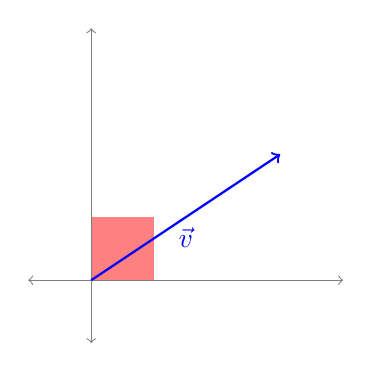
\begin{tikzpicture}[scale=0.8]
\fill[red!50!white] (0,0) rectangle (1,1);
\draw[thin,gray,<->] (-1,0)-- (4,0);
\draw[thin,gray,<->] (0,-1)-- (0,4);
\draw[thick,blue,->] (0,0) -- node[below] {$\vec{v}$} (3,2);
\end{tikzpicture}
\end{center}
  \begin{enumerate}[a)]
    \item 0
    \item 1
    \item 2
    \item 4
  \end{enumerate}
\end{activity}


\begin{activity}{5}
The transformations of the unit square by the
standard matrices \([\vec{v}\hspace{0.5em} \vec{w}]\) and
\([c\vec{v}\hspace{0.5em} \vec{w}]\) are illustrated below.
Describe the value of \(\det([c\vec{v}\hspace{0.5em} \vec{w}])\).
\begin{center}
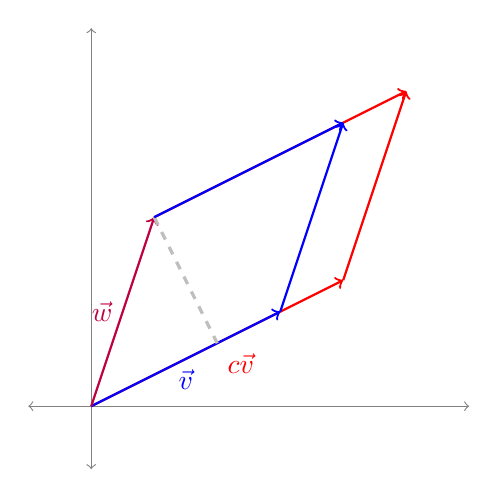
\begin{tikzpicture}[scale=0.8]
\draw[thin,gray,<->] (-1,0)-- (6,0);
\draw[thin,gray,<->] (0,-1)-- (0,6);
\draw[thick,red,->] (0,0) -- node[below right] {$c\vec{v}$}  (4,2);
\draw[thick,red,->] (1,3) -- (5,5);
\draw[thick,blue,->] (0,0) -- node[below] {$\vec{v}$} (3,1.5);
\draw[thick,purple,->] (0,0) -- node[left] {$\vec{w}$} (1,3);
\draw[lightgray,very thick,dashed] (1,3) -- (2,1);
\draw[thick,blue,->] (3,1.5) -- (4,4.5);
\draw[thick,blue,->] (1,3) -- (4,4.5);
\draw[thick,red,->] (4,2) -- (5,5);
\end{tikzpicture}
\end{center}
  \begin{enumerate}[a)]
    \item \(\det([\vec{v}\hspace{0.5em} \vec{w}])\)
    \item \(\det([\vec{v}\hspace{0.5em} \vec{w}])+c\)
    \item \(c\det([\vec{v}\hspace{0.5em} \vec{w}])\)
  \end{enumerate}
\end{activity}

\begin{activity}{5}
The transformations of unit squares by the
standard matrices \([\vec{u}\hspace{0.5em} \vec{w}]\), \([\vec{v}\hspace{0.5em} \vec{w}]\) and
\([\vec{u}+\vec{v}\hspace{0.5em} \vec{w}]\) are illustrated below.
Describe the value of \(\det([\vec{u}+\vec{v}\hspace{0.5em} \vec{w}])\).
\begin{center}
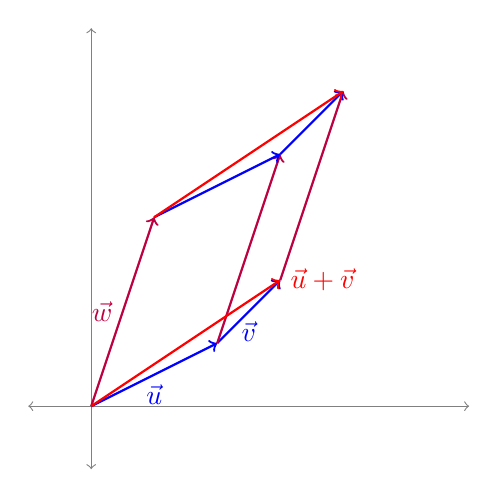
\begin{tikzpicture}[scale=0.8]
\draw[thin,gray,<->] (-1,0)-- (6,0);
\draw[thin,gray,<->] (0,-1)-- (0,6);
\draw[thick,blue,->] (0,0) -- node[below] {$\vec{u}$} (2,1);
\draw[thick,purple,->] (0,0) -- node[left] {$\vec{w}$} (1,3);
\draw[thick,blue,->] (2,1) -- node [below] {$\vec{v}$}(3,2);
\draw[thick,purple,->] (2,1) -- (3,4);
\draw[thick,purple,->] (3,2) -- (4,5);
\draw[thick,blue,->] (1,3) -- (3,4);
\draw[thick,blue,->] (3,4) -- (4,5);
\draw[thick,red,->] (0,0) --  (3,2)node[above,right] {$\vec{u}+\vec{v}$};
\draw[thick,red,->] (1,3) -- (4,5);
\end{tikzpicture}
\end{center}
  \begin{enumerate}[a)]
    \item
    \(\det([\vec{u}\hspace{0.5em} \vec{w}])=\det([\vec{v}\hspace{0.5em} \vec{w}])\)
    \item
    \(\det([\vec{u}\hspace{0.5em} \vec{w}])+\det([\vec{v}\hspace{0.5em} \vec{w}])\)
    \item
    \(\det([\vec{u}\hspace{0.5em} \vec{w}])\det([\vec{v}\hspace{0.5em} \vec{w}])\)
  \end{enumerate}
\end{activity}


\begin{definition}
The \term{determinant} is the unique function
\(\det:M_{n,n}\to\IR\) satisfying these  properties:
\begin{enumerate}
\item [P1:] $\det(I)=1$
\item [P2:] $\det(A)=0$ whenever two columns of the matrix are identical.
\item[P3:]
\(\det[\cdots\hspace{0.5em}c\vec{v}\hspace{0.5em}\cdots]=
c\det[\cdots\hspace{0.5em}\vec{v}\hspace{0.5em}\cdots]\), assuming no other columns change.
\item[P4:]
\(\det[\cdots\hspace{0.5em}\vec{v}+\vec{w}\hspace{0.5em}\cdots]=
\det[\cdots\hspace{0.5em}\vec{v}\hspace{0.5em}\cdots]+
\det[\cdots\hspace{0.5em}\vec{w}\hspace{0.5em}\cdots]\), assuming no other columns change.
\end{enumerate}

\vspace{1em}

Note that these last two properties together can be phrased as ``The determinant is linear in each column.''

\end{definition}


\begin{observation}
The determinant must also satisfy other properties.
Consider \(\det([\vec v \hspace{1em}\vec w+c \vec{v}])\) and
\(\det([\vec v\hspace{1em}\vec w])\).

\begin{center}
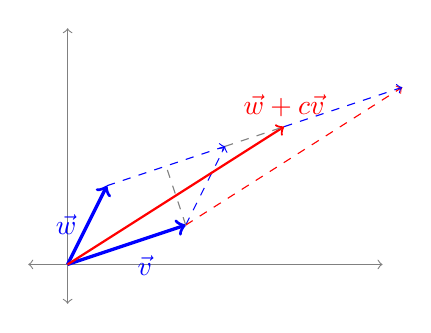
\begin{tikzpicture}[scale=0.5]
\draw[thin,gray,<->] (-1,0)-- (8,0);
\draw[thin,gray,<->] (0,-1)-- (0,6);
\draw[very thick,blue,->] (0,0) -- node[below right] {$\vec{v}$}  (3,1);
\draw[very thick,blue,->] (0,0) -- node[left] {$\vec{w}$} (1,2);
\draw[dashed,blue,->] (1,2) -- (4,3);
\draw[dashed,blue,->] (3,1) -- (4,3);
\draw[thick,red,->] (0,0) -- (5.5,3.5) node[above] {$\vec{w}+c\vec{v}$};
\draw[dashed,red,->] (3,1) -- (8.5,4.5);
\draw[dashed,blue,->] (5.5,3.5) -- (8.5,4.5);
\draw[thin,dashed,gray] (3,1) -- (2.5,2.5);
\draw[thin,dashed,gray] (4,3) -- (5.5,3.5);
\end{tikzpicture}
\end{center}

The base of both parallelograms is $\vec{v}$, while the height has not changed,
so the determinant does not change either. This can also be proven using the
other properties of the determinant:
  \begin{align*}
  \det([\vec{v}+c\vec{w}\hspace{1em}\vec{w}])
&=
  \det([\vec{v}\hspace{1em}\vec{w}])+
  \det([c\vec{w}\hspace{1em}\vec{w}])
\\ &=
  \det([\vec{v}\hspace{1em}\vec{w}])+
  c\det([\vec{w}\hspace{1em}\vec{w}])
\\ &=
  \det([\vec{v}\hspace{1em}\vec{w}])+
  c\cdot 0
\\ &=
  \det([\vec{v}\hspace{1em}\vec{w}])
  \end{align*}
\end{observation}

\begin{remark}
Swapping columns may be thought of as a reflection, which is represented by a negative
determinant. For example, the following matrices transform the unit square into
the same parallelogram, but the second matrix reflects its orientation.
\[
  A=\begin{bmatrix}2&3\\0&4\end{bmatrix}\hspace{1em}\det A=8\hspace{3em}
  B=\begin{bmatrix}3&2\\4&0\end{bmatrix}\hspace{1em}\det B=-8
\]
\begin{center}
\begin{tikzpicture}[scale=0.5]
\fill[red!50!white] (0,0) rectangle (1,1);
\draw[thin,gray,<->] (-4,0)-- (4,0);
\draw[thin,gray,<->] (0,-4)-- (0,4);
\draw[thick,blue,->] (0,0) -- node[below] {$A \vec{e}_1= \begin{bmatrix}2 \\ 0 \end{bmatrix}$}++ (2,0);
\draw[thick,blue,->] (0,0) -- ++(3,4) node[above] {$A \vec{e}_2 = \begin{bmatrix} 3 \\ 4 \end{bmatrix}$};
\draw[thick,red,->] (0,0) -- ++(1,0);
\draw[thick,red,->] (0,0) -- ++(0,1);
\draw[blue,dashed] (2,0) -- (5,4) -- (3,4);
\draw[red,dashed] (1,0) -- (1,1) -- (0,1);
\end{tikzpicture}
\begin{tikzpicture}[scale=0.5]
\fill[red!50!white] (0,0) rectangle (1,1);
\draw[thin,gray,<->] (-4,0)-- (4,0);
\draw[thin,gray,<->] (0,-4)-- (0,4);
\draw[thick,blue,->] (0,0) -- node[below] {$B \vec{e}_2= \begin{bmatrix}2 \\ 0 \end{bmatrix}$}++ (2,0);
\draw[thick,blue,->] (0,0) -- ++(3,4) node[above] {$B \vec{e}_1 = \begin{bmatrix} 3 \\ 4 \end{bmatrix}$};
\draw[thick,red,->] (0,0) -- ++(1,0);
\draw[thick,red,->] (0,0) -- ++(0,1);
\draw[blue,dashed] (2,0) -- (5,4) -- (3,4);
\draw[red,dashed] (1,0) -- (1,1) -- (0,1);
\end{tikzpicture}
\end{center}

\end{remark}


\begin{observation}
The fact that swapping columns multiplies determinants by a negative
may be verified by adding and subtracting columns.
\begin{align*}
  \det([\vec{v}\hspace{1em}\vec{w}])
&=
  \det([\vec{v}+\vec{w}\hspace{1em}\vec{w}])
\\ &=
  \det([\vec{v}+\vec{w}\hspace{1em}\vec{w}-(\vec{v}+\vec{w})])
\\ &=
  \det([\vec{v}+\vec{w}\hspace{1em}-\vec{v}])
\\ &=
  \det([\vec{v}+\vec{w}-\vec{v}\hspace{1em}-\vec{v}])
\\ &=
  \det([\vec{w}\hspace{1em}-\vec{v}])
\\ &=
  -\det([\vec{w}\hspace{1em}\vec{v}])
  \end{align*}
\end{observation}



\begin{fact}
  To summarize, we've shown that the column versions of the three row-reducing operations
  a matrix may be used to simplify a determinant in the following way:
  \begin{enumerate}[(a)]
  \item Multiplying a column by a scalar multiplies the
        determinant by that scalar:
        \[c\det([\cdots\hspace{0.5em}\vec{v}\hspace{0.5em} \cdots])=
        \det([\cdots\hspace{0.5em}c\vec{v}\hspace{0.5em} \cdots])\]
  \item Swapping two columns changes the sign of the determinant:
        \[\det([\cdots\hspace{0.5em}\vec{v}\hspace{0.5em}
        \cdots\hspace{1em}\vec{w}\hspace{0.5em} \cdots])=
        -\det([\cdots\hspace{0.5em}\vec{w}\hspace{0.5em}
        \cdots\hspace{1em}\vec{v}\hspace{0.5em} \cdots])\]
  \item Adding a multiple of a column to another column does not
        change the determinant:
        \[\det([\cdots\hspace{0.5em}\vec{v}\hspace{0.5em}
        \cdots\hspace{1em}\vec{w}\hspace{0.5em} \cdots])=
        \det([\cdots\hspace{0.5em}\vec{v}+c\vec{w}\hspace{0.5em}
        \cdots\hspace{1em}\vec{w}\hspace{0.5em} \cdots])\]
  \end{enumerate}
\end{fact}

\begin{activity}{5}
  The transformation given by the standard matrix \(A\) scales areas by
  \(4\), and the transformation given by the standard matrix \(B\) scales
  areas by \(3\). By what factor does the transformation given by the standard matrix
  \(AB\) scale areas?

\begin{center}
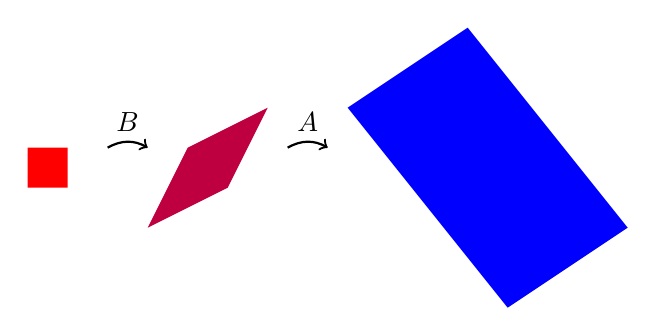
\begin{tikzpicture}[x=0.2in,y=0.2in]
\begin{scope}
\fill[red] (0,0) -- (1,0) -- (1,1) -- (0,1) -- (0,0);
\end{scope}
\draw[->,thick] (2,1) to[bend left=30] node[above] {\(B\)} (3,1);
\begin{scope}[shift={(3,-1)}]
\fill[purple] (0,0) -- (2,1) -- (3,3) -- (1,2) -- (0,0);
\end{scope}
\draw[->,thick] (6.5,1) to[bend left=30] node[above] {\(A\)} (7.5,1);
\begin{scope}[shift={(12,-3)}]
\fill[blue] (0,0) -- (-4,5) -- (-1,7) -- (3,2) -- (0,0);
\end{scope}
\end{tikzpicture}
\end{center}

  \begin{enumerate}[(a)]
  \item \(1\)
  \item \(7\)
  \item \(12\)
  \item Cannot be determined
  \end{enumerate}
\end{activity}

\begin{fact}
Since the transformation given by the standard matrix \(AB\) is obtained
by applying the transformations given by \(A\) and \(B\), it follows that 
\[\det(AB)=\det(A)\det(B)=\det(B)\det(A)=\det(BA)\]
\end{fact}

\begin{remark}
Recall that row operations may be produced by matrix multiplication.
\begin{itemize}
\item Multiply the first row of \(A\) by \(c\): \(
  \begin{bmatrix}
  c & 0 & 0 \\
  0 & 1 & 0 \\
  0 & 0 & 1
  \end{bmatrix}A
\)
\item Swap the first and second row of \(A\): \(
  \begin{bmatrix}
  0 & 1 & 0 \\
  1 & 0 & 0 \\
  0 & 0 & 1
  \end{bmatrix}A
\)
\item Add \(c\) times the third row to the first row of \(A\): \(
  \begin{bmatrix}
  1 & 0 & c \\
  0 & 1 & 0 \\
  0 & 0 & 1
  \end{bmatrix}A
\)
\end{itemize}
\end{remark}


\begin{fact}
The determinants of row operation matrices may be computed
by manipulating columns to reduce each matrix to the identity:
\begin{itemize}
\item Scaling a row: \(\det
  \begin{bmatrix}
  c & 0 & 0 \\
  0 & 1 & 0 \\
  0 & 0 & 1
  \end{bmatrix}
    =
  c\det
  \begin{bmatrix}
  1 & 0 & 0 \\
  0 & 1 & 0 \\
  0 & 0 & 1
  \end{bmatrix}
    =
  c
\)
\item Swapping rows: \(\det
  \begin{bmatrix}
  0 & 1 & 0 \\
  1 & 0 & 0 \\
  0 & 0 & 1
  \end{bmatrix}
    =
  -1\det
  \begin{bmatrix}
  1 & 0 & 0 \\
  0 & 1 & 0 \\
  0 & 0 & 1
  \end{bmatrix}
    =
  -1
\)
\item Adding a row multiple to another row: \(\det
  \begin{bmatrix}
  1 & 0 & c \\
  0 & 1 & 0 \\
  0 & 0 & 1
  \end{bmatrix}
    =
  \det
  \begin{bmatrix}
  1 & 0 & c-1c \\
  0 & 1 & 0-0c \\
  0 & 0 & 1-0c
  \end{bmatrix}
    =
  \det(I)=1
\)
\end{itemize}
\end{fact}

\begin{activity}{5}
Consider the row operation \(R_1+4R_3\to R_1\) applied as follows to show
\(A\sim B\):
\[
A=\begin{bmatrix}1&2&3\\4&5&6\\7&8&9\end{bmatrix}
  \sim
\begin{bmatrix}1+4(7)&2+4(8)&3+4(9)\\4&5&6\\7&8&9\end{bmatrix}=B
\]
\begin{enumerate}[(a)]
\item Find a matrix \(R\) such that \(B=RA\), by applying the same row operation to 
\(I=\begin{bmatrix}1&0&0\\0&1&0\\0&0&1\end{bmatrix}\).
\item Find \(\det R\) by comparing with the previous slide.
\item If \(C \in M_{3,3}\) is a matrix with \(\det(C)= -3\), find 
\[\det(RC)=\det(R)\det(C).\]
\end{enumerate}
\end{activity}

\begin{activity}{5}
Consider the row operation \(R_1\leftrightarrow R_3\) applied as follows to show
\(A\sim B\):
\[
A=\begin{bmatrix}1&2&3\\4&5&6\\7&8&9\end{bmatrix}
  \sim
\begin{bmatrix}7&8&9\\4&5&6\\1&2&3\end{bmatrix}=B
\]
\begin{enumerate}[(a)]
\item Find a matrix \(R\) such that \(B=RA\), by applying the same row operation to \(I\).
\item If \(C \in M_{3,3}\) is a matrix with \(\det(C)= 5\), find \(\det(RC)\).
\end{enumerate}
\end{activity}

\begin{activity}{5}
Consider the row operation \(3R_2\to R_2\) applied as follows to show
\(A\sim B\):
\[
A=\begin{bmatrix}1&2&3\\4&5&6\\7&8&9\end{bmatrix}
  \sim
\begin{bmatrix}1&2&3\\3(4)&3(5)&3(6)\\7&8&9\end{bmatrix}=B
\]
\begin{enumerate}[(a)]
\item Find a matrix \(R\) such that \(B=RA\).
\item If \(C \in M_{3,3}\) is a matrix with \(\det(C)= -7\), find \(\det(RC)\).
\end{enumerate}
\end{activity}


\begin{remark}
  Recall that the column versions of the three row-reducing operations
  a matrix may be used to simplify a determinant:
  \begin{enumerate}[(a)]
  \item Multiplying columns by scalars:
        \[\det([\cdots\hspace{0.5em}c\vec{v}\hspace{0.5em} \cdots])=
        c\det([\cdots\hspace{0.5em}\vec{v}\hspace{0.5em} \cdots])\]
  \item Swapping two columns:
        \[\det([\cdots\hspace{0.5em}\vec{v}\hspace{0.5em}
        \cdots\hspace{1em}\vec{w}\hspace{0.5em} \cdots])=
        -\det([\cdots\hspace{0.5em}\vec{w}\hspace{0.5em}
        \cdots\hspace{1em}\vec{v}\hspace{0.5em} \cdots])\]
  \item Adding a multiple of a column to another column:
        \[\det([\cdots\hspace{0.5em}\vec{v}\hspace{0.5em}
        \cdots\hspace{1em}\vec{w}\hspace{0.5em} \cdots])=
        \det([\cdots\hspace{0.5em}\vec{v}+c\vec{w}\hspace{0.5em}
        \cdots\hspace{1em}\vec{w}\hspace{0.5em} \cdots])\]
  \end{enumerate}
\end{remark}
\begin{remark}
The determinants of row operation matrices may be computed
by manipulating columns to reduce each matrix to the identity:
\begin{itemize}
\item Scaling a row: \(  
  \begin{bmatrix}
  1 & 0 & 0 \\
  0 & c & 0 \\
  0 & 0 & 1
  \end{bmatrix}
\)
\item Swapping rows: \(
  \begin{bmatrix}
  0 & 1 & 0 \\
  1 & 0 & 0 \\
  0 & 0 & 1
  \end{bmatrix}
\)
\item Adding a row multiple to another row: \(
  \begin{bmatrix}
  1 & 0 & 0 \\
  0 & 1 & c \\
  0 & 0 & 1
  \end{bmatrix}
\)
\end{itemize}
\end{remark}
\begin{fact}
Thus we can also use row operations to simplify determinants:
\begin{enumerate}
\item Multiplying rows by scalars:
  \(\det\begin{bmatrix}\vdots\\cR\\\vdots\end{bmatrix}=
  c\det\begin{bmatrix}\vdots\\R\\\vdots\end{bmatrix}\)
\item Swapping two rows:
  \(\det\begin{bmatrix}\vdots\\R\\\vdots\\S\\\vdots\end{bmatrix}=
  -\det\begin{bmatrix}\vdots\\S\\\vdots\\R\\\vdots\end{bmatrix}\)
\item Adding multiples of rows to other rows:
  \(\det\begin{bmatrix}\vdots\\R\\\vdots\\S\\\vdots\end{bmatrix}=
  \det\begin{bmatrix}\vdots\\R+cS\\\vdots\\S\\\vdots\end{bmatrix}\)
\end{enumerate}
\end{fact}



\begin{observation}
  So we may compute the determinant of \(\begin{bmatrix} 2 & 4 \\ 2 & 3 \end{bmatrix}\) 
  by manipulating its rows/columns to reduce the matrix to \(I\):

  \begin{align*}
    \det\begin{bmatrix} 2 & 4 \\ 2 & 3 \end{bmatrix}
      &=
    2 \det \begin{bmatrix} 1 & 2 \\ 2 & 3 \end{bmatrix}\\
      &=
    %2 \det \begin{bmatrix} 1 & 2 \\ 2-2(1) & 3-2(2)\end{bmatrix}=
    2 \det \begin{bmatrix} 1 & 2 \\ 0 & -1 \end{bmatrix}\\
      &=
    %2(-1) \det \begin{bmatrix} 1 & -2 \\ 0 & +1 \end{bmatrix}=
    -2 \det \begin{bmatrix} 1 & -2 \\ 0 & 1 \end{bmatrix}\\
      &=
    %-2 \det \begin{bmatrix} 1+2(0) & -2+2(1) \\ 0 & 1\end{bmatrix} =
    -2 \det \begin{bmatrix} 1 & 0 \\ 0 & 1 \end{bmatrix}\\
      &=
    %-2\det I = 
	%-2(1) = 
	-2
  \end{align*}
\end{observation}

\begin{remark}
So we see that row reducing all the way into RREF gives us a method of computing determinants!

\vspace{1em}

However, we learned in module E that this can be tedious for large matrices.  Thus, we will try
to figure out how to turn the determinant of a larger matrix
into the determinant of a smaller matrix.
\end{remark}



\begin{activity}{5}
  The following image illustrates the transformation of the unit cube
  by the matrix
  $\begin{bmatrix} 3 & 1 & 0 \\  1 & 1 & 1 \\  0 & 0 & 1\end{bmatrix}$.

  \begin{center}
  \begin{tikzpicture}
  \fill[purple!50!white] (0,0,0) -- (1,0,1) -- (4,0,2) -- (3,0,1) -- (0,0,0);
  \draw[thin,gray,->] (0,0,0) -- (3,0,0);
  \draw[thin,gray,->] (0,0,0) -- (0,2,0);
  \draw[thin,gray,->] (0,0,0) -- (0,0,2);
  %(y,z,x)
  \draw[blue] (1,0,1) -- (4,0,2) -- (3,0,1);
  \draw[blue] (1,1,0) -- (2,1,1) -- (5,1,2) -- (4,1,1) -- (1,1,0);
  \draw[blue] (1,0,1) -- +(1,1,0);
  \draw[blue] (4,0,2) -- +(1,1,0);
  \draw[blue] (3,0,1) -- +(1,1,0);

  \draw[purple,thick,->] (0,0,0) -- (1,1,0)
    node[above left]{\tiny$\begin{bmatrix} 0 \\ 1 \\ 1\end{bmatrix}$};
  \draw[purple,thick,->] (0,0,0) -- (1,0,1)
    node[below]{\tiny$\begin{bmatrix} 1 \\ 1 \\ 0\end{bmatrix}$};
  \draw[purple,thick,->] (0,0,0) -- (3,0,1)
    node[above right]{\tiny$\begin{bmatrix} 3 \\ 1 \\ 0\end{bmatrix}$};
  \draw[purple,dashed,very thick] (0,0,0) -- node[left] {\tiny\(h=1\)} (0,1,0);
  \end{tikzpicture}
  \end{center}
  Recall that for this solid \(V=Bh\), where \(h\) is the height of the solid 
  and \(B\) is the area of its parallelogram base.
  So what must its volume be?
\begin{multicols}{4}
\begin{enumerate}[(a)]
\item $\det \begin{bmatrix} 3 & 1 \\ 1 & 1 \end{bmatrix}$
\item $\det \begin{bmatrix} 3 & 1 \\ 1 & 0 \end{bmatrix}$
\item $\det \begin{bmatrix} 3 & 1 \\ 0 & 1 \end{bmatrix}$
\item $\det \begin{bmatrix} 1 & 1 \\ 0 & 1 \end{bmatrix}$
\end{enumerate}
\end{multicols}
\end{activity}

\begin{fact}
If row \(i\) contains all zeros except for a \(1\) on the 
main (upper-left to lower-right) diagonal, 
then both column and row \(i\)
may be removed without changing the value of the determinant.
\[
  \det \begin{bmatrix}
    3 & \textcolor{red}{2} & -1 & 3 \\
    \textcolor{red}{0} & \textcolor{red}{1} 
      & \textcolor{red}{0} & \textcolor{red}{0} \\
    -1 & \textcolor{red}{4} & 1 & 0 \\
    5 & \textcolor{red}{0} & 11 & 1
  \end{bmatrix} =
  \det \begin{bmatrix}
    3 & -1 & 3 \\
    -1 & 1 & 0 \\
    5 & 11 & 1
  \end{bmatrix}
\]
Since row and column operations affect the determinants in the same
way, the same technique works for a column of all zeros except for
a \(1\) on the main diagonal.
\[
  \det \begin{bmatrix}
    3 & \textcolor{red}{0} & -1 & 5 \\
    \textcolor{red}{2} & \textcolor{red}{1} & \textcolor{red}{4} & 
       \textcolor{red}{0} \\
    -1 & \textcolor{red}{0} & 1 & 11 \\
    3 & \textcolor{red}{0} & 0 & 1
  \end{bmatrix} =
  \det \begin{bmatrix}
    3 & -1 & 5 \\
    -1 & 1 & 11 \\
    3 & 0 & 1
  \end{bmatrix}
\] 
\end{fact}


\begin{activity}{5}
  Remove an appropriate row and column of  
  $\det \begin{bmatrix} 1 & 0 & 0 \\ 1 & 5 & 12 \\ 3 & 2 & -1 \end{bmatrix}$
  to simplify the determinant to a \(2\times 2\) determinant.
\end{activity}

\begin{activity}{5}
  Simplify
  \(\det \begin{bmatrix} 0 & 3 & -2 \\ 2 & 5 & 12 \\ 0 & 2 & -1 \end{bmatrix}\)
  to a multiple of a \(2\times 2\) determinant by first doing the following:
  \begin{itemize}
    \item Factor out a \(2\) from a column.
    \item Swap rows or columns to put a \(1\) on the main diagonal.
  \end{itemize}
\end{activity}

\begin{activity}{5}
  Simplify
  \(\det \begin{bmatrix} 4 & -2 & 2 \\ 3 & 1 & 4 \\ 1 & -1 & 3\end{bmatrix}\)
  to a multiple of a \(2\times 2\) determinant by first doing the following:
  \begin{itemize}
    \item Use row/column operations to create two zeroes in the same row or column.
    \item Factor/swap as needed to get a row/column of all zeroes except 
      a \(1\) on the main diagonal.
  \end{itemize}
\end{activity}


\begin{observation}
Using row/column operations, you can introduce zeros
and reduce dimension to whittle down the determinant of a large
matrix to a determinant of a smaller matrix.

\begin{align*}
    \det\begin{bmatrix} 
      4 & 3 & 0 & 1 \\ 
      2 & -2 & 4 & 0 \\ 
      -1 & 4 & 1 & 5 \\ 
      2 & 8 & 0 & 3 
    \end{bmatrix}
  &=
    \det\begin{bmatrix} 
      4 & 3 & \textcolor{red}{0} & 1 \\ 
      6 & -18 & \textcolor{red}{0} & -20 \\ 
      \textcolor{red}{-1} & \textcolor{red}{4} & 
        \textcolor{red}{1} & \textcolor{red}{5} \\ 
      2 & 8 & \textcolor{red}{0} & 3 
    \end{bmatrix}
  =
    \det\begin{bmatrix} 
      4 & 3 & 1 \\ 
      6 & -18 & -20 \\ 
      2 & 8 & 3 
    \end{bmatrix}
  \\&=\dots=
    -2\det\begin{bmatrix}
      \textcolor{red}{1} & \textcolor{red}{3} & \textcolor{red}{4} \\ 
      \textcolor{red}{0} & 21 & 43 \\ 
      \textcolor{red}{0} & -1 & -10 
    \end{bmatrix}
  =
    -2\det\begin{bmatrix} 21 & 43 \\ -1 & -10 \end{bmatrix}
  \\&= \dots=
    -2\det\begin{bmatrix}
      -167 & \textcolor{red}{21} \\
      \textcolor{red}{0} & \textcolor{red}{1}
    \end{bmatrix}
   = -2\det[-167]
  \\&=-2(-167)\det(I)=
    334
\end{align*} 
\end{observation}

\begin{activity}{10}
  Compute 
  \(
    \det\begin{bmatrix} 
      2 & 3 & 5 & 0 \\ 
      0 & 3 & 2 & 0 \\ 
      1 & 2 & 0 & 3 \\ 
      -1 & -1 & 2 & 2 
    \end{bmatrix}
  \) by using any combination of row/column operations.
\end{activity}

\begin{observation}
Another option is to take advantage of the fact that the determinant is linear 
in each row or column.  This approach is called
\term{Laplace expansion} or \term{cofactor expansion}. 

For example, since 
\textcolor{blue}{\(
  \begin{bmatrix} 1 & 2 & 4 \end{bmatrix} 
= 
  1\begin{bmatrix} 1 & 0 & 0 \end{bmatrix}
+
  2\begin{bmatrix} 0 & 1 &  0 \end{bmatrix}
+
  4\begin{bmatrix} 0  & 0 & 1 \end{bmatrix}
\)},

  \begin{align*}
\det \begin{bmatrix} 2 & 3 & 5  \\ -1 & 3 & 5 \\ \textcolor{blue}{1} & \textcolor{blue}{2} & \textcolor{blue}{4} \end{bmatrix} &=
\textcolor{blue}{1}\det \begin{bmatrix} 2 & 3 & 5  \\ -1 & 3 & 5 \\ \textcolor{blue}{1} & \textcolor{blue}{0} & \textcolor{blue}{0} \end{bmatrix} +
\textcolor{blue}{2}\det \begin{bmatrix} 2 & 3 & 5  \\ -1 & 3 & 5 \\ \textcolor{blue}{0} & \textcolor{blue}{1} & \textcolor{blue}{0} \end{bmatrix} +
\textcolor{blue}{4}\det \begin{bmatrix} 2 & 3 & 5  \\ -1 & 3 & 5 \\ \textcolor{blue}{0} & \textcolor{blue}{0} & \textcolor{blue}{1} \end{bmatrix} \\
&= -1\det \begin{bmatrix}  5 & 3 & 2 \\ 5 & 3 & -1 \\ 0 & 0 & 1 \end{bmatrix} 
-2\det \begin{bmatrix} 2 & 5 & 3  \\ -1 & 5 & 3 \\ 0 & 0 & 1 \end{bmatrix} +
4\det \begin{bmatrix} 2 & 3 & 5  \\ -1 & 3 & 5 \\ 0 & 0 & 1 \end{bmatrix} \\
&= -\det \begin{bmatrix} 5 & 3 \\ 5 & 3 \end{bmatrix} 
-2 \det \begin{bmatrix} 2 & 5 \\ -1 & 5 \end{bmatrix}
+4 \det \begin{bmatrix} 2 & 3 \\ -1 & 3 \end{bmatrix}
\end{align*}

\end{observation}

\begin{observation}
Applying Laplace expansion to a \(2 \times 2\) matrix yields a short formula you may have seen:
\[
  \det \begin{bmatrix} \textcolor{blue}{a} & \textcolor{blue}{b} \\ c & d \end{bmatrix}
=
  \textcolor{blue}{a}\det \begin{bmatrix} \textcolor{blue}{1} & \textcolor{blue}{0} \\ 
    c & d \end{bmatrix} 
+ 
  \textcolor{blue}{b} \det \begin{bmatrix} \textcolor{blue}{0} & \textcolor{blue}{1} \\ 
    c & d \end{bmatrix} 
=
  a\det \begin{bmatrix} \textcolor{red}{1} & \textcolor{red}{0} \\ 
    \textcolor{red}{c} & d \end{bmatrix} 
-
  b \det \begin{bmatrix} \textcolor{red}{1} & \textcolor{red}{0} \\ 
    \textcolor{red}{d} & c \end{bmatrix} 
= 
  ad-bc
.\]

\vspace{1em}

There are formulas for the determinants of larger matrices,
but they can be pretty tedious to use. For example, writing out a
formula for a \(4\times 4\) determinant would require 24 different terms!

\[
   \det\begin{bmatrix}
     a_{11} & a_{12} & a_{13} & a_{14} \\
     a_{21} & a_{22} & a_{23} & a_{24} \\
     a_{31} & a_{32} & a_{33} & a_{34} \\
     a_{41} & a_{42} & a_{43} & a_{44}
   \end{bmatrix}
     =
   a_{11}(a_{22}(a_{33}a_{44}-a_{43}a_{34})-a_{23}(a_{32}a_{44}-a_{42}a_{34})+\dots)+\dots
\]

So this is why we either use Laplace expansion or row/column operations directly.
\end{observation}

\begin{activity}{10}
  Use Laplace expansion to compute 
  \(
    \det\begin{bmatrix} 
      2 & 2 & 1 & 0 \\ 
      0 & 3 & 2 & -1 \\ 
      3 & 2 & 0 & 3 \\ 
      0 & -3 & 2 & -2 
    \end{bmatrix}
  \).
\end{activity}

\begin{activity}{5}
Based on what we've done today, which technique is easier for computing determinants?
\begin{enumerate}[(a)]
\item Memorizing formulas.
\item Using row/column operations.
\item Laplace expansion.
\item Some other technique (be prepared to describe it).
\end{enumerate}
\end{activity}

\begin{activity}{10}
  Use your preferred technique to compute 
  \(
    \det\begin{bmatrix} 
      4 & -3 & 0 & 0 \\ 
      1 & -3 & 2 & -1 \\ 
      3 & 2 & 0 & 3 \\ 
      0 & -3 & 2 & -2 
    \end{bmatrix}
  \).
\end{activity}

\begin{activity}{5}
  An invertible matrix \(M\) and its inverse \(M^{-1}\) are given below:
 
  \[
    M=\begin{bmatrix}1&2\\3&4\end{bmatrix}
  \hspace{2em}
    M^{-1}=\begin{bmatrix}-2&1\\3/2&-1/2\end{bmatrix}
  \]

\vspace{1em}

  Which of the following is equal to \(\det(M)\det(M^{-1})\)?

\begin{enumerate}[a)]
\item \(-1\)
\item \(0\)
\item \(1\)
\item \(4\)
\end{enumerate}
\end{activity}

\begin{fact}
  \begin{itemize}
\item   For every invertible matrix \(M\),
  \[
    \det(M)\det(M^{-1})= \det(I)=1
  \]
  so \(\det(M^{-1})=\frac{1}{\det(M)}\).

\item  Furthermore,
  a square matrix \(M\) is invertible if and only if \(\det(M)\not=0\).
  \end{itemize}
\end{fact}

\begin{observation}
Consider the linear transformation \(A : \IR^2 \rightarrow \IR^2\) 
given by the matrix \(A = \begin{bmatrix} 2 & 2 \\ 0 & 3 \end{bmatrix}\).

\begin{center}
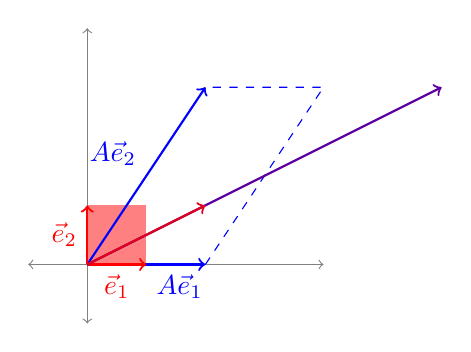
\begin{tikzpicture}[scale=0.75]
\fill[red!50] (0,0) rectangle (1,1);
\draw[thin,gray,<->] (-1,0)-- (4,0);
\draw[thin,gray,<->] (0,-1)-- (0,4);
\draw[thick,blue,->] (0,0) -- node[below right] {$A \vec{e}_1$}++ (2,0);
\draw[thick,red,->] (0,0) -- node[below] {$\vec{e}_1$}++ (1,0);
\draw[thick,blue,->] (0,0) -- node[above left] {$A \vec{e}_2$}++(2,3);
\draw[thick,red,->] (0,0) -- node[left] {$\vec{e}_2$}++ (0,1);
\draw[blue,dashed] (2,0) -- (4,3) -- (2,3);
\draw[purple!50!blue,thick,->] (0,0) -- (6,3);
\draw[purple!50!red,thick,->] (0,0) -- (2,1);
\end{tikzpicture}
\end{center}
It is easy to see geometrically that
\[
  A\begin{bmatrix}1 \\ 0 \end{bmatrix} = 
  \begin{bmatrix} 2 & 2 \\ 0 & 3 \end{bmatrix}\begin{bmatrix}1 \\ 0 \end{bmatrix}=
  \begin{bmatrix}2 \\ 0 \end{bmatrix}= 
  2 \begin{bmatrix}1 \\ 0 \end{bmatrix}
\]

It is less obvious (but easily checked once you find it) that
\[
  A\begin{bmatrix} 2 \\ 1 \end{bmatrix} = 
  \begin{bmatrix} 2 & 2 \\ 0 & 3 \end{bmatrix}\begin{bmatrix}2 \\ 1 \end{bmatrix}=
  \begin{bmatrix} 6 \\ 3 \end{bmatrix} = 
  3\begin{bmatrix} 2 \\ 1 \end{bmatrix}
\]
\end{observation}

\begin{definition}
Let $A \in M_{n,n}$.
An \term{eigenvector} for \(A\) 
is a vector $\vec{x} \in \IR^n$ such that $A\vec{x}$ is parallel to $\vec{x}$.

\begin{center}
\begin{tikzpicture}[scale=0.75]
\fill[gray!50] (0,0) rectangle (1,1);
\draw[thin,gray,<->] (-1,0)-- (4,0);
\draw[thin,gray,<->] (0,-1)-- (0,4);
\draw[thick,blue,->] (0,0) -- node[below right] {$A \vec{e}_1=2\vec e_1$}++ (2,0);
\draw[thick,red,->] (0,0) -- node[below] {$\vec{e}_1$}++ (1,0);
\draw[thick,gray,->] (0,0) -- node[above left] {$A \vec{e}_2$}++(2,3);
\draw[thick,gray,->] (0,0) -- node[left] {$\vec{e}_2$}++ (0,1);
\draw[gray,dashed] (2,0) -- (4,3) -- (2,3);
\draw[purple!50!blue,thick,->] (0,0) -- (6,3) 
  node [below right] {\(
   A\begin{bmatrix}2\\1\end{bmatrix}
     =
   3\begin{bmatrix}2\\1\end{bmatrix}
  \)};
\draw[purple!50!red,thick,->] (0,0) -- (2,1)
  node [above] {\(\begin{bmatrix}2\\1\end{bmatrix}\)};
\end{tikzpicture}
\end{center}

In other words, $A\vec{x}=\lambda \vec{x}$ for some scalar $\lambda$. 
If \(\vec x\not=\vec 0\), then we say \(\vec x\) is a \term{nontrivial eigenvector}
and we call this \(\lambda\) an \term{eigenvalue} of \(A\).
\end{definition}

\begin{activity}{5}
Finding the eigenvalues \(\lambda\) that satisfy
\[
  A\vec x=\lambda\vec x=\lambda(I\vec x)=(\lambda I)\vec x
\]
for some nontrivial eigenvector \(\vec x\) is equivalent to finding 
nonzero solutions for the matrix equation
\[
  (A-\lambda I)\vec x =\vec 0
.\]
Which of the following must be true for any eigenvalue?
\begin{enumerate}[(a)]
\item The \textbf{kernel} of the transformation with standard matrix \(A-\lambda I\)
must contain \textbf{the zero vector}, so \(A-\lambda I\) is \textbf{invertible}.
\item The \textbf{kernel} of the transformation with standard matrix \(A-\lambda I\)
must contain \textbf{a non-zero vector}, so \(A-\lambda I\) is \textbf{not invertible}.
\item The \textbf{image} of the transformation with standard matrix \(A-\lambda I\)
must contain \textbf{the zero vector}, so \(A-\lambda I\) is \textbf{invertible}.
\item The \textbf{image} of the transformation with standard matrix \(A-\lambda I\)
must contain \textbf{a non-zero vector}, so \(A-\lambda I\) is \textbf{not invertible}.
\end{enumerate}
\end{activity}

\begin{fact}
  The eigenvalues \(\lambda\) for a matrix \(A\) are the values
  that make \(A-\lambda I\) non-invertible.

  \vspace{1em}

  Thus the eigenvalues \(\lambda\) for a matrix \(A\)
  are the solutions to
  the equation \[\det(A-\lambda I)=0.\]
\end{fact}

\begin{definition}
The expression \(\det(A-\lambda I)\) is called
\term{characteristic polynomial} of \(A\). \\

\vspace{1em} 

For example, when
\(A=\begin{bmatrix}1 & 2 \\ 3 & 4\end{bmatrix}\), we have

\[
  A-\lambda I=
  \begin{bmatrix}1 & 2 \\ 3 & 4\end{bmatrix}-
  \begin{bmatrix}\lambda & 0 \\ 0 & \lambda\end{bmatrix}=
  \begin{bmatrix}1-\lambda & 2 \\ 3 & 4-\lambda\end{bmatrix}
\]

\ \\
Thus the characteristic polynomial of \(A\) is
\[
  \det\begin{bmatrix}1-\lambda & 2 \\ 3 & 4-\lambda\end{bmatrix}
=
  (1-\lambda)(4-\lambda)-(2)(3)
=
  \lambda^2-5\lambda-2
\]
and its eigenvalues are the solutions to \(\lambda^2-5\lambda-2=0\).
\end{definition}

\begin{activity}{10}
  Compute $\det(A-\lambda I)$ using co-factor expansion or another technique
  to find the characteristic polynomial of
  \(A=\begin{bmatrix} 6 & -2 & 1 \\ 0 & -5 & 0 \\ -4 & 2 & 1 \end{bmatrix}\).
\end{activity}

\begin{activity}{10}
Let $A = \begin{bmatrix} 5 & 2 \\ -3 & -2 \end{bmatrix}$.
\begin{subactivity}
Compute $\det (A-\lambda I)$ to determine the characteristic polynomial of $A$.
\end{subactivity}
\begin{subactivity}
Set this characteristic polynomial equal to zero and factor to determine the eigenvalues of $A$.
\end{subactivity}
\end{activity}

\begin{activity}{10}
  Find all the eigenvalues for the matrix
  $A=\begin{bmatrix} 3 & -3 \\ 2 & -4 \end{bmatrix}$.
\end{activity}

\begin{activity}{10}
It's possible to show that \(-2\) is an eigenvalue for
\(\begin{bmatrix}-1&4&-2\\2&-7&9\\3&0&4\end{bmatrix}\).

\vspace{1em}

Compute the kernel of the transformation with standard matrix
\[
  A-(-2)I
    =
  \begin{bmatrix} \unknown & 4&-2 \\ 2 & \unknown & 9\\3&0&\unknown \end{bmatrix}
\] 
to find all the eigenvectors \(\vec x\) such that \(A\vec x=-2\vec x\).
\end{activity}

\begin{definition}
  Since the kernel of a linear map is a subspace
  of \(\IR^n\), and the kernel obtained from \(A-\lambda I\)
  contains all the eigenvectors associated with \(\lambda\),
  we call this kernel the \term{eigenspace} of \(A\) associated with \(\lambda\).
\end{definition}


\begin{activity}{10}
Find a basis for the eigenspace for the matrix
\(
  \begin{bmatrix}
    5 & -2 & 0 & 4 \\ 6 & -2 & 1 & 5 \\ -2 & 1 & 2 & -3 \\ 4 & 5 & -3 & 6
  \end{bmatrix}
\)
associated with the eigenvalue \(1\).
\end{activity}


